\section{Arquitectura del sistema}
\label{sec:arquitectura}

Fresh es una aplicación cliente--servidor. El mismo proceso de Python sirve la interfaz web y la API, de modo que basta con abrir \texttt{http://localhost:8000}. La figura~\ref{fig:arquitectura} muestra las capas.

\begin{figure}[ht]
\centering
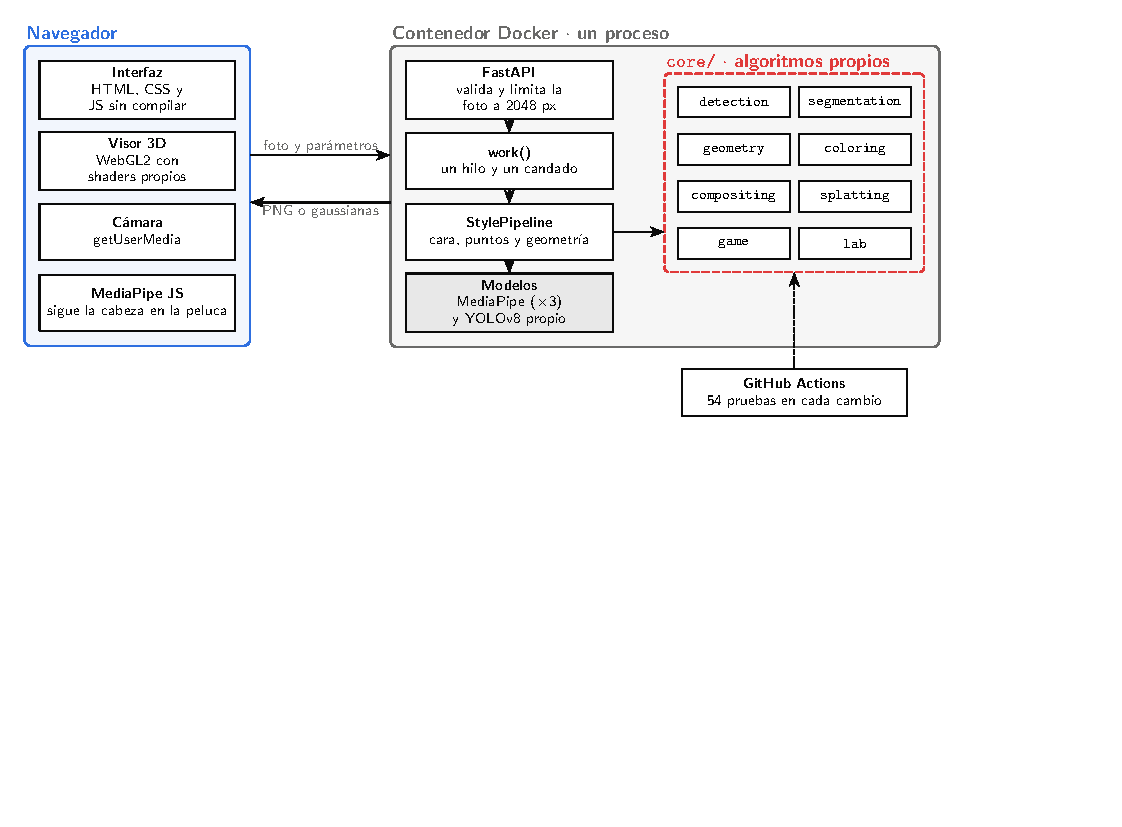
\includegraphics[width=\linewidth]{diagrama_arquitectura.pdf}
\caption{Arquitectura de Fresh. El navegador envía la foto y los parámetros; un único proceso de FastAPI, dentro de un contenedor Docker, pasa cada llamada por \texttt{work()} al pipeline y devuelve la imagen procesada o las gaussianas que dibuja el visor WebGL2.}
\label{fig:arquitectura}
\end{figure}

\subsection{Servidor}

El servidor está escrito en Python con FastAPI \cite{fastapi}, OpenCV \cite{bradski2000} y NumPy \cite{harris2020}. Se organiza en tres niveles:
\begin{itemize}
  \item \textbf{API} (\archivo{api/routes.py}): valida parámetros, decodifica la imagen, la reduce a un lado máximo de 2048~px y devuelve un PNG o datos binarios. No contiene lógica gráfica.
  \item \textbf{Orquestación} (\archivo{core/pipeline.py}): la clase \texttt{StylePipeline} carga los modelos una sola vez y encadena los pasos comunes de cada herramienta: cara, puntos, geometría de la cabeza y probabilidades de segmentación.
  \item \textbf{Módulos} (\archivo{core/*}): cada técnica vive en su propio paquete, sin depender de la API, y es lo que prueban los tests unitarios.
\end{itemize}

\textbf{Un solo proceso, a propósito.} El modo en vivo, la prueba de la peluca y el juego guardan estado entre cuadros: el ancla de la cara, el color del pelo y la ronda en curso. Por eso el servidor corre un único proceso de \texttt{uvicorn}; con dos, cada cuadro caía en uno distinto y el juego alternaba entre dos partidas. Cada llamada al \emph{pipeline} se ejecuta en un hilo aparte detrás de un candado, así el servidor sigue respondiendo mientras procesa una foto y los modelos nunca se usan desde dos hilos a la vez.

\subsection{Interfaz}

La interfaz no usa \emph{frameworks} ni compilación:
\begin{itemize}
  \item \archivo{index.html} define los paneles;
  \item \archivo{app.js} llama a la API de cada herramienta;
  \item \archivo{ui.js} implementa la navegación, la foto compartida, la combinación de looks, la ficha y las sugerencias;
  \item \archivo{splat3d.js} es el visor de gaussianas en WebGL2 \cite{khronos2017}.
\end{itemize}
Los datos personales (looks guardados) se quedan en el \texttt{localStorage} del navegador.

\subsection{Flujo de una petición}

Por ejemplo, al aplicar un degradado medio:
\begin{enumerate}
  \item el navegador envía \texttt{POST /api/haircut} con la foto, \texttt{style=mid-fade} y la intensidad;
  \item el servidor detecta la cara, calcula los 478 puntos y los convierte al formato de 68 puntos, construye la geometría de la cabeza y segmenta el pelo;
  \item el módulo \archivo{compositing/haircut.py} renderiza el corte sobre un recorte de la cabeza a una resolución de trabajo fija y lo devuelve a la resolución original;
  \item la interfaz muestra el resultado en el comparador antes/después.
\end{enumerate}
La lista completa de \emph{endpoints} está en el anexo~\ref{sec:anexo-api}.
